\section{问题分析与解决方案}

\par{} 在本次设计和调试的过程中,我们遇到了硬件和软件上的种种问题,虽然没有出现十分严重的问题,但依然每天的调试过程中也遇到了一些不顺利的现象,这些问题的解决带给了我们许多在电子设计方面的经验。



\subsection{硬件问题分析}

\par{} \textbf{1.虚焊共地问题}
\par{}首先在硬件方面,我们出现最多的问题便是系统不够稳定,表现为有时系统不能够驱动Arduino,又或者在接线完成后未通电情况下会出现检测模块指示灯亮的情况。而排查的思路也较为清晰,由于指示灯亮,自然的知道指示灯两端存在电位差,那么观测各个点的电位便能够很快的发现,某些模块的GND端并不严格的为0,而是出现了例如1.8V的电势差,虽不能驱动模块稳定工作,但已足够点亮LED,因此我们排查出在焊接板的地线引出端,各个地线我们通过拉锡连焊在一起,但发现可能有锡与导线间存在接触不良或虚焊导致出现模块不共地现象。解决时将其共地端重新连焊,保证万能板上的各个模块共地,立刻解决了问题。

\par{} \textbf{2.电池盒地线内部断路}

\par{} 问题的现象和上述共地问题相似,是在电池连接上Arduino后DHT11的LED指示灯亮,但这次由于具有上次共地问题的经验,经过排查能够很显然的发现,检测模块所在万能板共地没有出现问题。而电池连接上Arduino板后便出现指示灯亮的问题。并且,打开电源后,各个检测模块都没有在工作。
\par{}经过长时间的排查后我们发现是问题存在于电池与Arduino板间,起初以为是电池没电,无法驱动Arduino板正常工作,但万用表直接测量电池输出在8V左右,足以驱动Arduino板,因此我们不得不剪短了原本焊接在一起的电池和电源管理电路,单独看看是否电池能够驱动Arduino,后来发现果然不能够驱动,但发现电池与电池线共地并没有问题,Arduino板的共地也没有问题,经过和助教一起排查后确定是电池盒上焊接的Arduino供电口的地线内部出现接触不良的问题,导致共地出现错误,驱动出现问题,更换了电池盒便立刻解决问题。

\par{} \textbf{3.低通滤波参数设置问题}

\par{} 我们起初在对模块单独调试时,针对于PM2.5的检测模块,也即GP2Y1050,由于我们利用示波器观测其模拟量输出,存在高频噪声,因此需要经过低通滤波器,而GP2Y1050的原理在之前也已经提到,是由LED照亮后根据散射光强来确定污染物浓度的,datasheet中推荐我们用Arduino去驱动传感器中的LED进行闪烁,周期为10ms,而高电平持续时间为0.32ms,并且建议在时隔0.28ms后进行读数,如下图\ref{imgn}所示:
\begin{figure}[H]
  \centering
  \includegraphics[width = 0.618\textwidth]{GP2Y.png}
  \caption{灰尘传感器驱动时序}
  \label{imgn}
\end{figure}

\par{} 而我们起初将VCVS低通滤波的中心赫兹定在100Hz附近,因为我们认为采样的信号在100Hz,但实际在面包板上测试后发现,传感器读到的读数始终为0,这才发现可能是传感器根本没有工作,原因是经过低通滤波器后将驱动LED闪烁的信号滤除,这结合信号与系统的知识可以知道,我们驱动信号相当于是时间常数为0.32ms的矩形窗,而经过傅里叶变换后可知其主瓣频率宽度为$\frac{1}{\tau}$,也即是3.125kHz,因此我们把中心频率修改为3.8kHz左右时便解决了问题,PM2.5模块便立刻可以正常工作。

\par{} \textbf{4.焊接布局问题}
\par{} 在本次的设计中,由于焊接布局不是十分合理,导致后来调试时出现了接线十分复杂,并且容易断线难以调试的现象,并且为最后装箱造成了困难。
\par{} 接线效果如下图所示:
\begin{figure}[H]
  \centering
  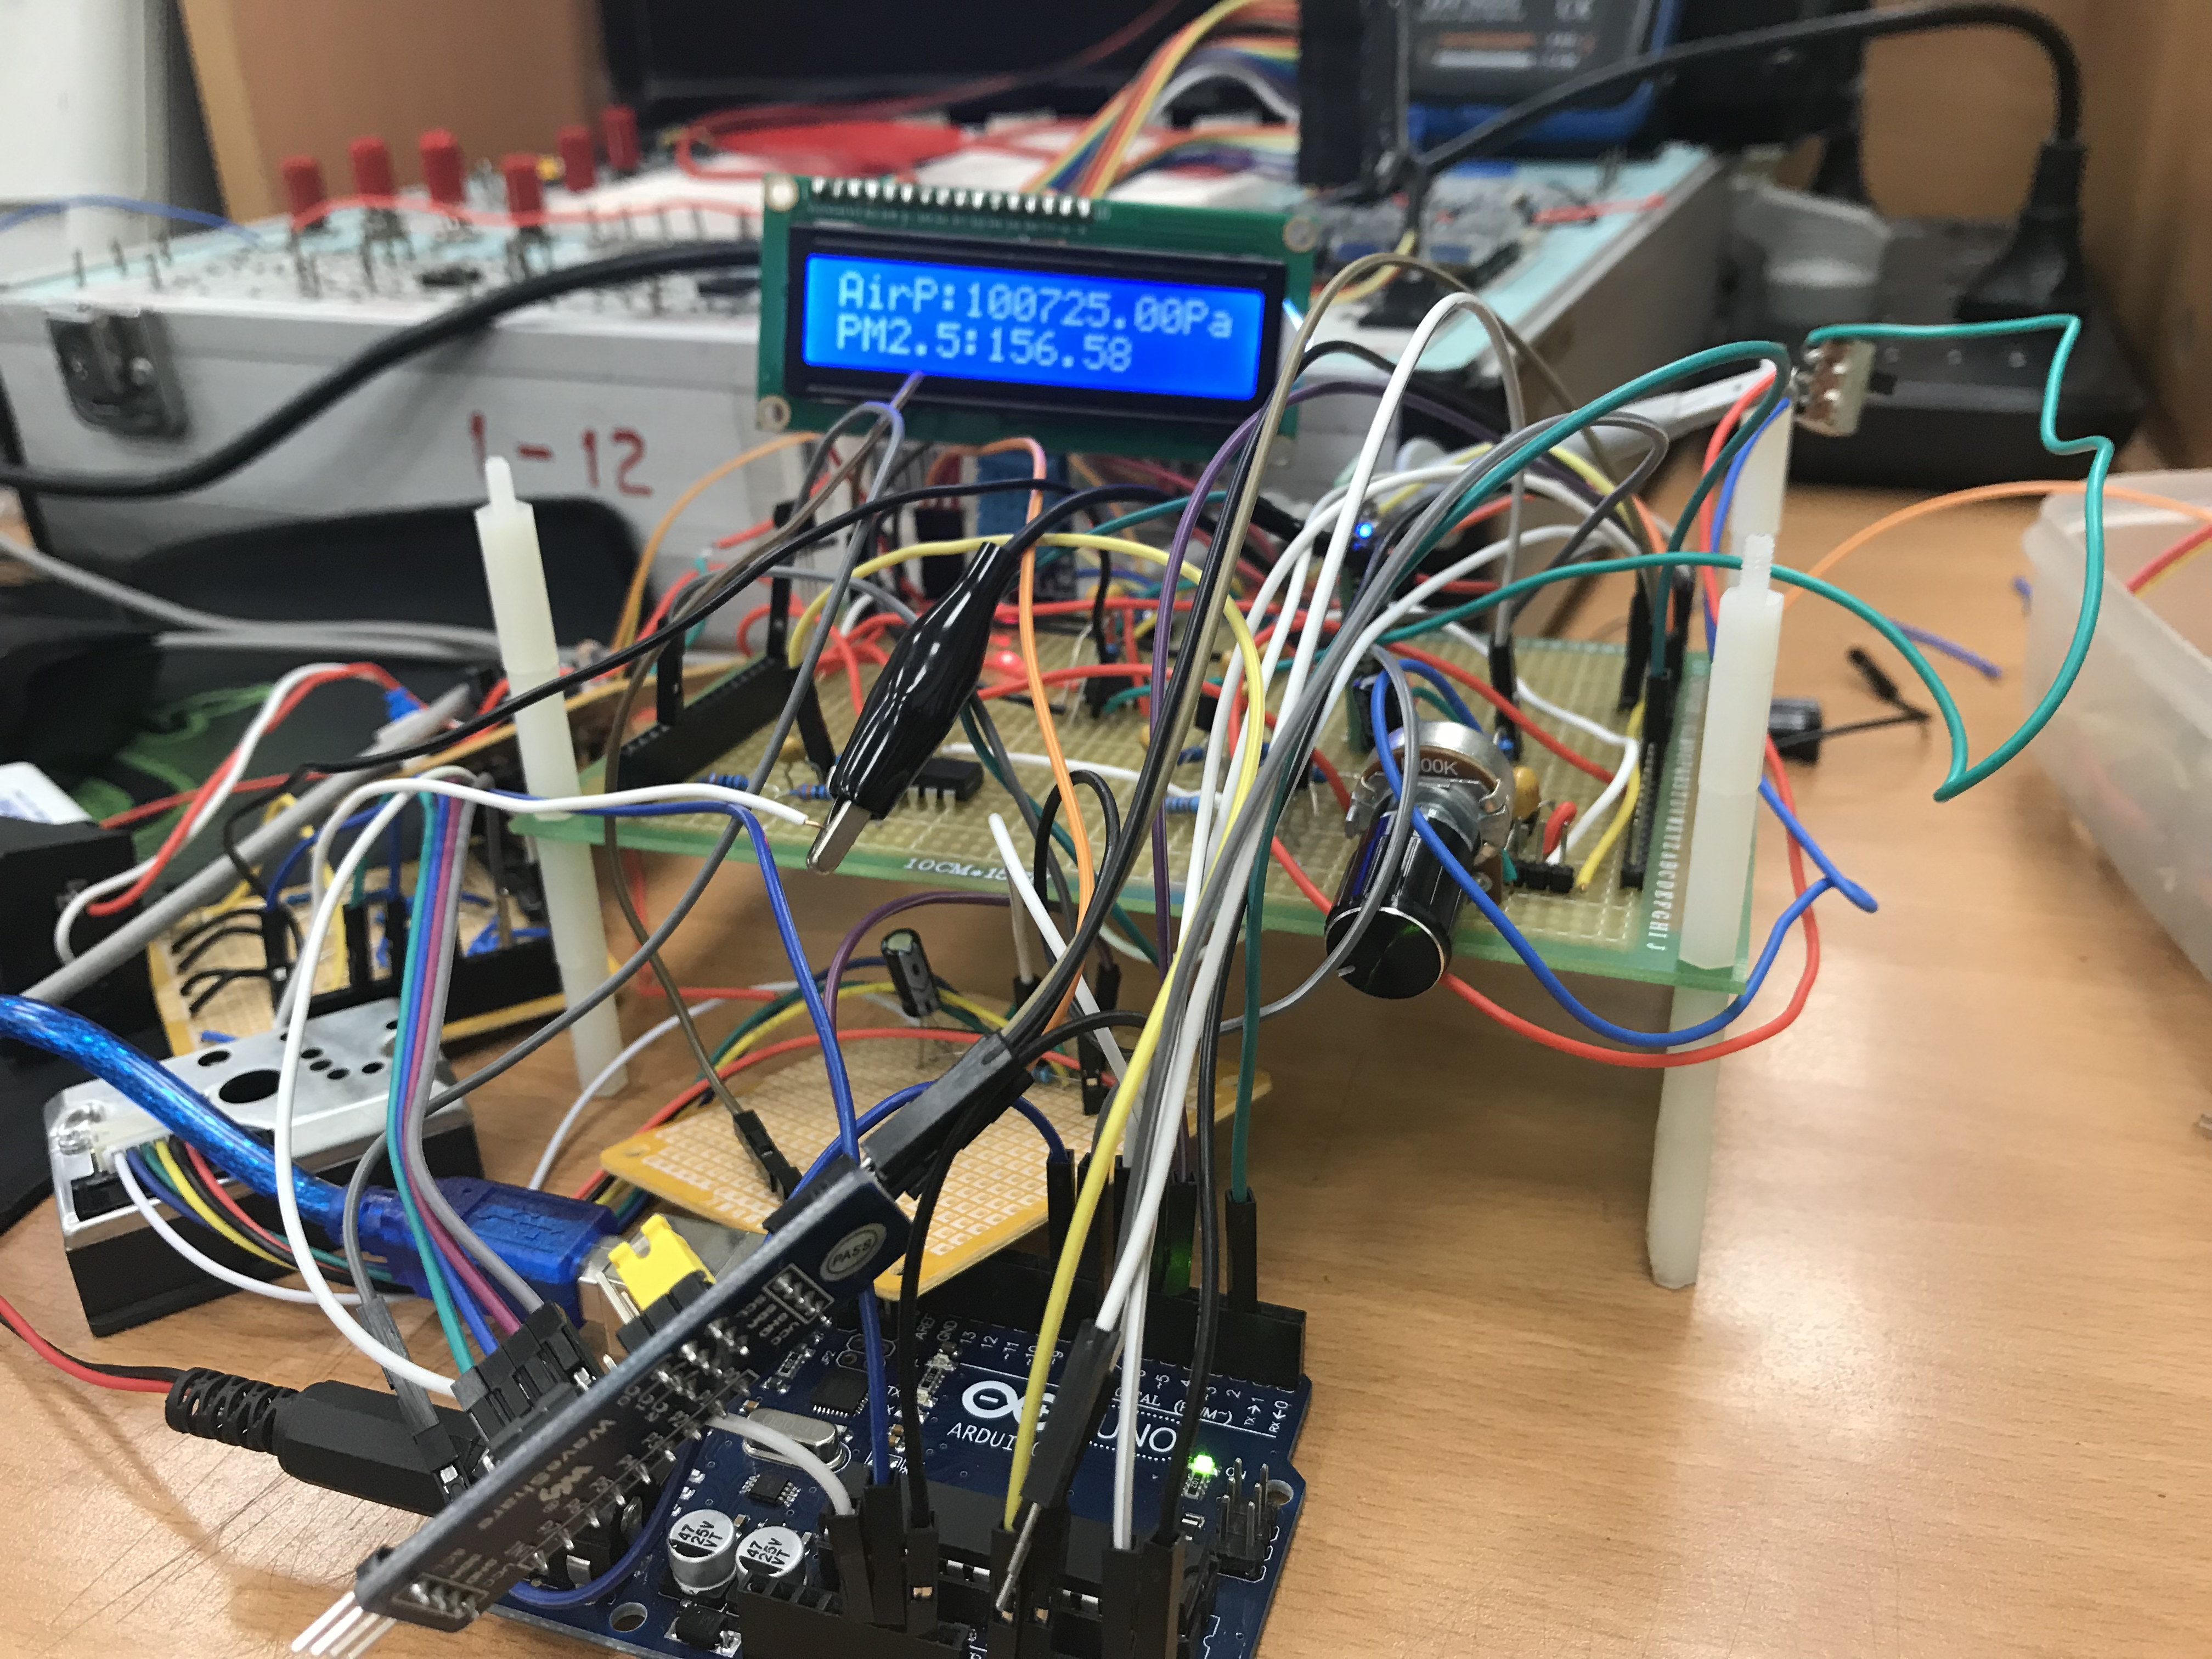
\includegraphics[width = 0.618\textwidth]{jiexian.jpg}
  \caption{实际接线图}
\end{figure}

\par{} 可以看出接线时十分复杂,极易将杜邦线错接或中途出现短接,这是由于我在焊接引出数据端时并不在板子的同一侧,以及引出VCC和GND过少,之后重新将DATA的引出规划在一侧,并且将VCC和GND和DATA在同一侧通过排针引出,便改善了这个问题。同时这个问题也提醒了我们在之后类似的设计中,例如万能板的焊接,走线采用统一的方式既能保证板子的整洁,也便于之后的调试。
\par{} \textbf{5.PCB制作问题}
\par{} 我们组曾在第一周尝试为电源管理模块制作PCB,而我们利用立创EDA制作了简单的PCB文件,如下图所示:
\begin{figure}[H]
  \centering
  \includegraphics[width = 0.618\textwidth]{PCB.png}
  \caption{PCB制作}
\end{figure}
\par{} 而之后在PCB制作完成后对自锁按键开关进行打孔的过程中,由于焊盘直径较小,将焊盘打没,则在焊接时锡直接流到了其他铜板上,无法有效的焊接自锁按键,最终PCB板作废。之后我们反思到首先是电源管理电路并不复杂,利用万能板会更方便一些,制作PCB耗时耗力,并且我们也吸取了经验,需要修改系统库中元件对于焊盘大小的设定,将焊盘设置够大以至于我们能够进行方便的打孔和焊接。

\par{} \textbf{6.Arduino板IO口资源紧张问题}
\par{} 由于我们的测量模块较多,需要与Arduino板直接相连的数据较多,因此显然的出现了IO口不够用的情况,这也是我们在设计时便考虑到的问题。而解决方法便是我们通过深入理解I2C协议,将机械键盘控制模块经过IO转I2C转接板,使得气压模块,LCD显示模块和机械键盘模块均通过I2C协议传送数据,极大的节省了IO口的使用。
\subsection{软件问题分析}
\par{} 在软件层面,除了在利用控制字编写状态机出现的逻辑或语法上的小错误外,我们主要问题是动态内存和程序空间不足。Arduino UNO板在动态内存使用超过75\%时便会报警,而内存的限制也限制了我们在功能和模块上的添加,因此我们也不得不相伴发节省动态内存和程序空间,至少能够达到我们的基本要求。

\par{} 而分析动态内存和程序存储空间不足的原因,可以从以下的三个方面得出:
\begin{itemize}
\item 部分类库冗余度高,占用了大量空间。
\item 主程序中的各分立的中间变量占用空间较多。
\item 打印数据前缀、单位等字符串常量也占用空间。
\end{itemize}

\par{} 因此对应于以上的三个方面,我们首先去精简类库,例如DHT11类库进行精简与修改,其次我们换用BMP的官方库,去除了一些冗余的变量和函数,提高系统效率。其次用更贴近底层和数字电路所学的知识进行系统的简化,节约内存。设计化简状态字,并$uint8\_t$类型存储,在状态判定转换时,依数电、计原所学,多用位操作以提升效率。此外,用PROGMEM后缀,将字符存在flashrom中能够有效的减少动态内存的占用,基于以上的设计和优化,我们最终在动态内存73\%的边缘完成了项目的设计。